\documentclass[pdftex]{article}
\usepackage[utf8]{inputenc}
\usepackage{adjustbox}
\usepackage{caption}
\usepackage[margin=0cm]{geometry}
\usepackage{pgfplots}
\pgfplotsset{compat=1.17}
\begin{document}
   \begin{figure}
   \centering
   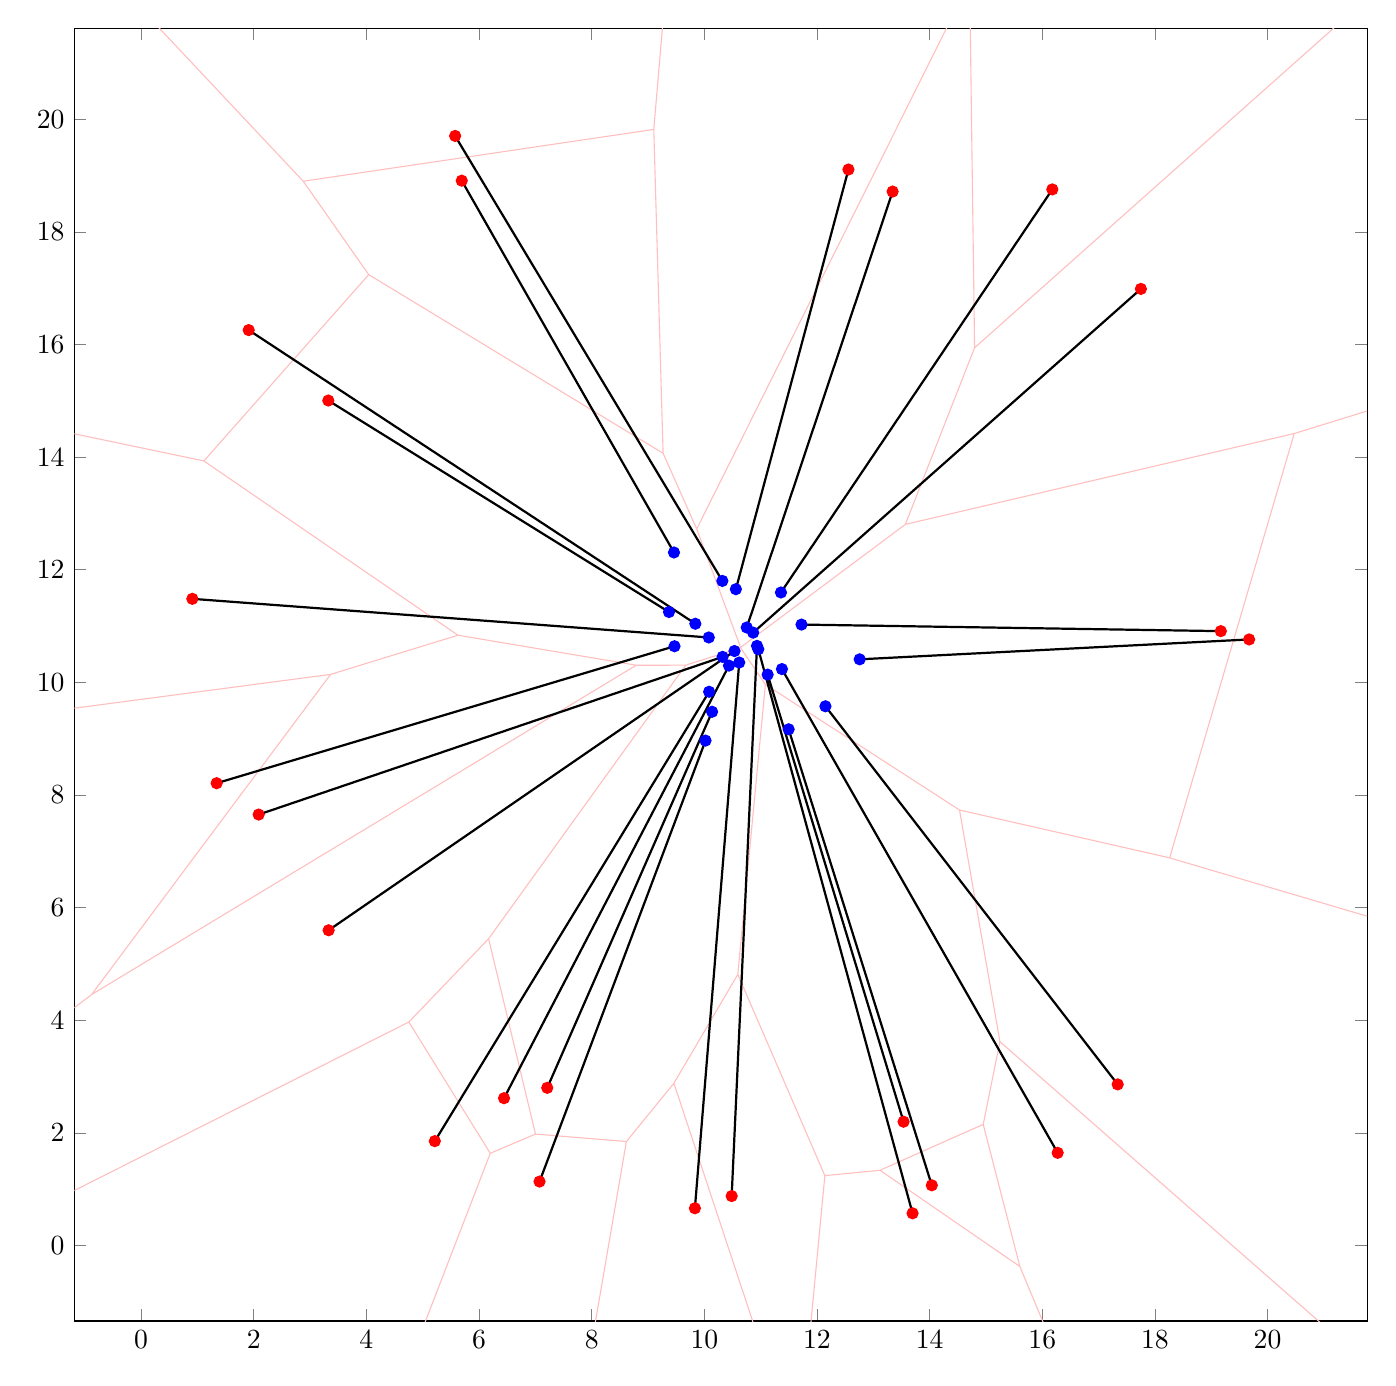
\begin{tikzpicture}
      \begin{axis}[
          axis equal, width=18cm, height=18cm
      ]
      \addplot [only marks, blue] table { 
10.9583 10.5892
10.5353 10.5565
11.7253 11.0266
9.37246 11.2495
12.15 9.57603
10.0851 9.83372
9.4608 12.3067
10.0791 10.7977
10.0211 8.96685
10.3203 11.8016
10.3243 10.4531
11.3602 11.5963
10.9349 10.6479
10.1379 9.47848
11.3777 10.2366
10.7527 10.9749
10.5599 11.6548
12.7579 10.4097
10.4374 10.2985
11.4967 9.16796
10.8668 10.8838
11.1239 10.1381
9.84036 11.0413
9.47031 10.642
10.6192 10.3526
 };
      \addplot [only marks,  red] table { 
12.5585 19.1056
3.32951 5.59952
17.3384 2.8631
1.34159 8.21023
17.7506 16.986
13.6967 0.574697
2.08744 7.6535
19.6726 10.7626
13.3429 18.7144
3.32407 15.0043
1.9107 16.2551
7.07408 1.13759
19.1699 10.9102
6.44392 2.61796
5.57557 19.7016
13.5371 2.20023
10.4852 0.880032
16.178 18.7526
0.909967 11.4836
7.21094 2.80213
9.83243 0.663789
5.69295 18.9078
16.2729 1.64818
5.21494 1.85541
14.0384 1.07159
 };
      \addplot [no markers, update limits=false,  red!25] table { 
-34.378262 21.375339
1.114436 13.931409

-15.689118 38.641830
2.878967 18.897272

3.364305 10.142085
-0.879305 4.456930

3.364305 10.142085
-40.689377 4.333214

3.364305 10.142085
5.626497 10.837542

-0.879305 4.456930
-13.767809 -5.356996

-0.879305 4.456930
8.791619 10.305071

-13.767809 -5.356996
4.753930 3.970038

12.858967 63.831114
9.102365 19.817532

18.154048 57.746938
14.710527 22.438651

38.199411 36.772468
14.798077 15.940961

51.472910 23.992120
20.472936 14.418261

10.673033 -46.724795
11.663372 -3.769878

27.122974 -28.018379
15.601907 -0.369528

38.191591 -16.500097
15.247606 3.622064

51.874778 -3.047340
18.261083 6.885072

14.798077 15.940961
14.710527 22.438651

14.798077 15.940961
13.568522 12.805398

14.710527 22.438651
9.865168 12.723162

1.114436 13.931409
5.626497 10.837542

1.114436 13.931409
4.041816 17.239268

5.626497 10.837542
8.791619 10.305071

8.791619 10.305071
9.669990 10.305579

-5.511454 -28.692222
6.199817 1.639743

1.931188 -37.069142
8.616095 1.848701

13.118139 1.338494
14.951092 2.152623

13.118139 1.338494
15.601907 -0.369528

13.118139 1.338494
12.139922 1.242449

14.951092 2.152623
15.601907 -0.369528

14.951092 2.152623
15.247606 3.622064

15.247606 3.622064
14.530545 7.734133

20.472936 14.418261
13.568522 12.805398

20.472936 14.418261
18.261083 6.885072

13.568522 12.805398
10.643473 10.621412

18.261083 6.885072
14.530545 7.734133

10.643473 10.621412
9.865168 12.723162

10.643473 10.621412
10.641856 10.615157

9.865168 12.723162
9.268020 14.067691

14.530545 7.734133
11.083977 9.963053

2.878967 18.897272
4.041816 17.239268

2.878967 18.897272
9.102365 19.817532

4.041816 17.239268
9.268020 14.067691

9.268020 14.067691
9.102365 19.817532

11.663372 -3.769878
12.139922 1.242449

11.663372 -3.769878
9.459560 2.882743

12.139922 1.242449
10.594227 4.815629

8.616095 1.848701
9.459560 2.882743

8.616095 1.848701
7.002390 1.981381

9.459560 2.882743
10.594227 4.815629

10.594227 4.815629
11.083977 9.963053

11.083977 9.963053
10.641856 10.615157

10.641856 10.615157
9.669990 10.305579

9.669990 10.305579
6.169782 5.448977

4.753930 3.970038
6.169782 5.448977

4.753930 3.970038
6.199817 1.639743

6.169782 5.448977
7.002390 1.981381

7.002390 1.981381
6.199817 1.639743


 };
      \addplot [no markers, thick] table { 
10.9583 10.5892
13.6967 0.574697

10.5353 10.5565
3.32951 5.59952

11.7253 11.0266
19.1699 10.9102

9.37246 11.2495
3.32407 15.0043

12.15 9.57603
17.3384 2.8631

10.0851 9.83372
5.21494 1.85541

9.4608 12.3067
5.69295 18.9078

10.0791 10.7977
0.909967 11.4836

10.0211 8.96685
7.07408 1.13759

10.3203 11.8016
5.57557 19.7016

10.3243 10.4531
2.08744 7.6535

11.3602 11.5963
16.178 18.7526

10.9349 10.6479
10.4852 0.880032

10.1379 9.47848
7.21094 2.80213

11.3777 10.2366
16.2729 1.64818

10.7527 10.9749
13.3429 18.7144

10.5599 11.6548
12.5585 19.1056

12.7579 10.4097
19.6726 10.7626

10.4374 10.2985
6.44392 2.61796

11.4967 9.16796
14.0384 1.07159

10.8668 10.8838
17.7506 16.986

11.1239 10.1381
13.5371 2.20023

9.84036 11.0413
1.9107 16.2551

9.47031 10.642
1.34159 8.21023

10.6192 10.3526
9.83243 0.663789
 };
      \end{axis}
   \end{tikzpicture}
   \caption*{Instance 25\_25\_E\_0 - exact\_subcubic\_1bad\_novoronoi }
   \end{figure}
\end{document}
